
\section{Experimental Setup Details}
\label{app:experimental_setup}

\subsection{Data Construction and Split}
\label{app:data_construction}

\paragraph{Persona Collection.}
We collect a diverse set of 2{,}100 character persona profiles spanning multiple domains, including game characters, film and television characters, and real-world figures, split into a 2{,}000-persona training set and a 100-persona held-out test set. As illustrated in Fig.~\ref{fig:persona_distribution}, the test personas cover five major categories: Fictional (43\%), Celebrities (29\%), Social (14\%), Creatures (9\%), and Others (5\%), demonstrating that our evaluation is domain-agnostic and generalizable across diverse character types.

\begin{figure}[t]
  \centering
  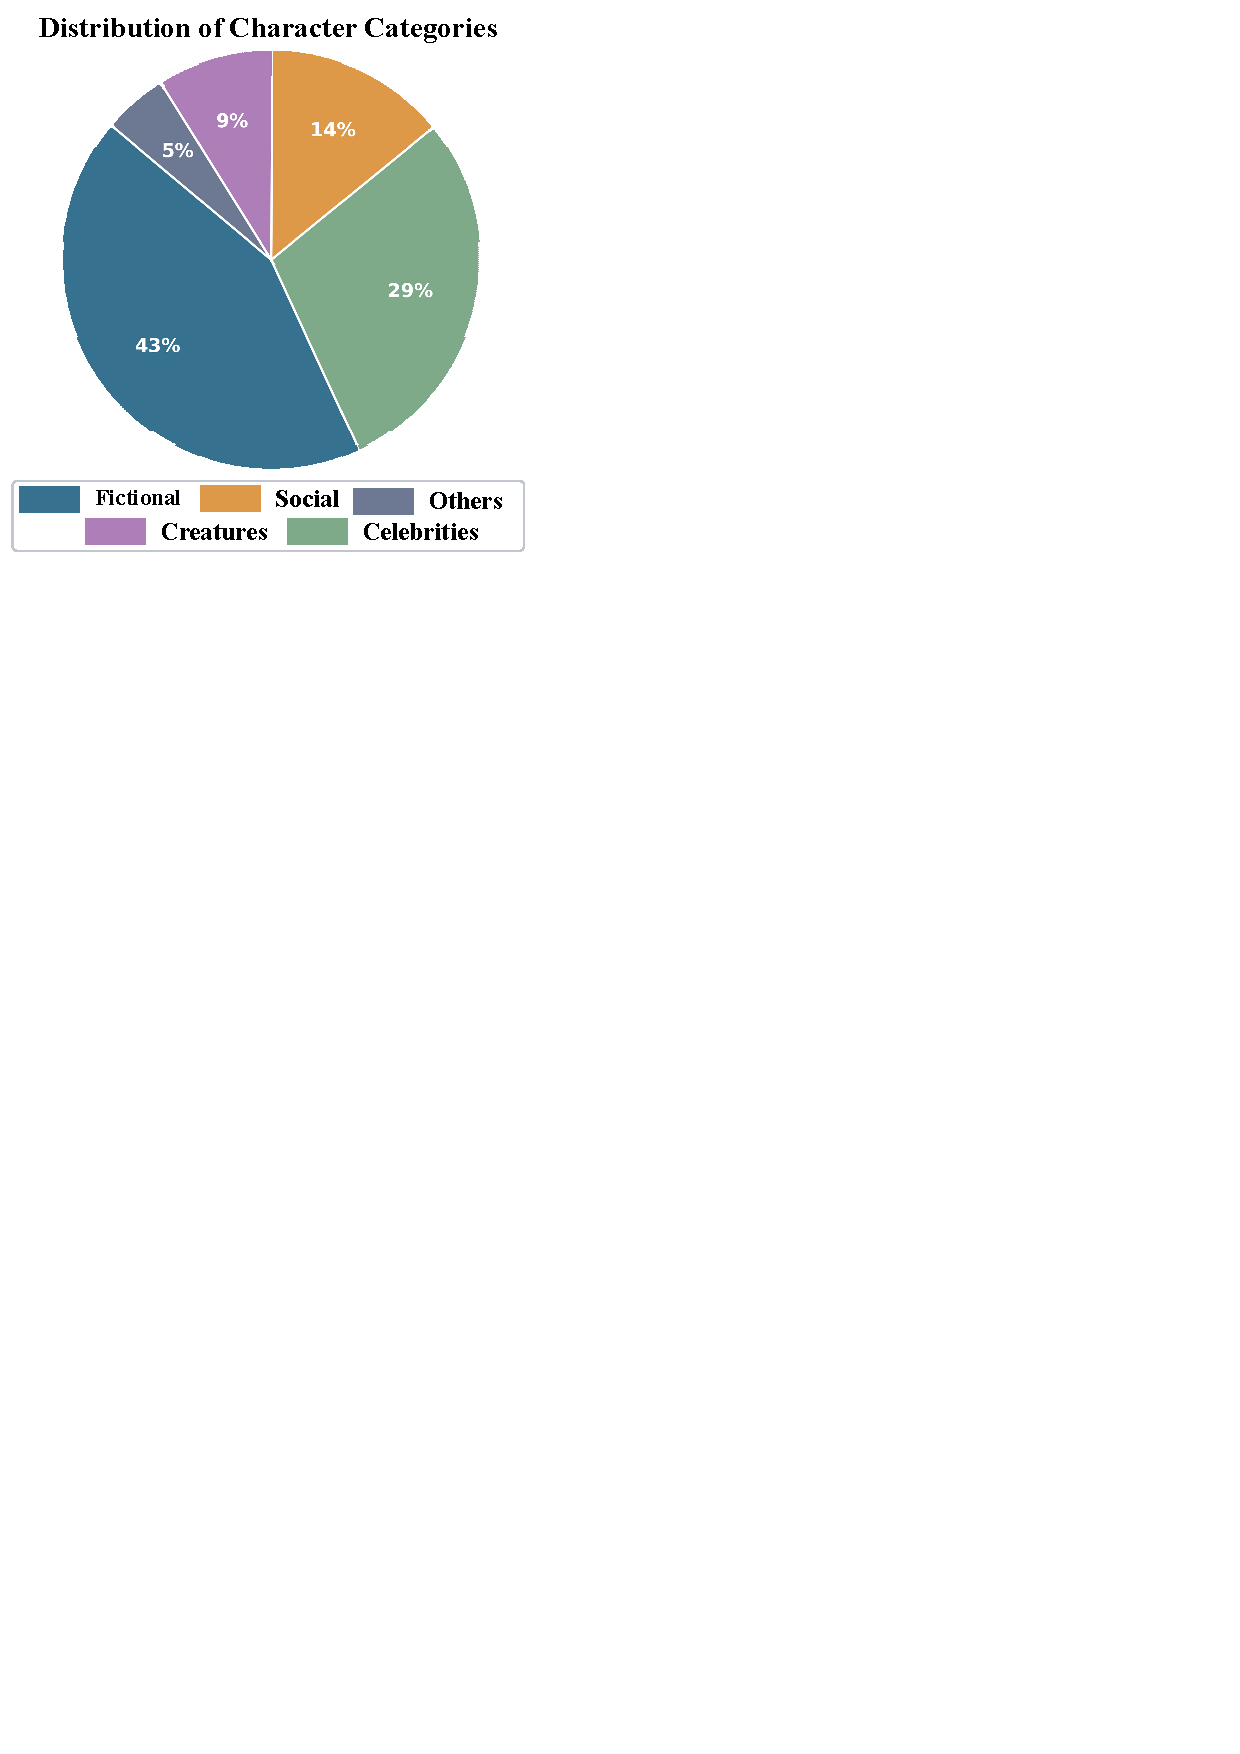
\includegraphics[width=\columnwidth, trim = 0 20cm 11.8cm 0, clip]{latex/Image/appendix-persona-pie-0520.pdf}

  \caption{Distribution of character categories in the test persona set.}
  \label{fig:persona_distribution}
\end{figure}


\paragraph{SFT Data Construction.}
For supervised fine-tuning, we construct one 50-turn trajectory for each of the 2{,}000 training personas using the multi-turn lookahead search in Section~\ref{sec:stage1}. The search uses a segment length of $T=10$ turns and $K=5$ sequential steps. At each step, $N_s=2$ candidate character agents are sampled from a global pool of $N=5$ models (Gemini-3-Pro, Claude Sonnet 4.6, GPT-5.4, Qwen-Plus-Character, and Doubao-1.5-Pro-Character). Both candidates continue from the same committed prefix and interact with the Doubao-1.5-Pro-Character user simulator for 10 turns. The higher-scoring segment is appended to the committed trajectory. The resulting 2{,}000 reward-optimized trajectories are used for SFT.

% For supervised fine-tuning, we construct a 50-turn dialogue trajectory for each of the 2{,}000 training personas using the Reward-Driven Trajectory Construction via Multi-turn Lookahead Search procedure described in Section~\ref{sec:train}. Specifically, with a chunk size of $T=10$ turns, the process advances in 5 steps. At each step, 2 candidate character agents are sampled from a diverse pool of 5 (Gemini-3-pro, Claude Sonnet 4.6, GPT-5.4, Qwen-plus-character, and Doubao-1.5-pro-character) to perform chunk-level rollouts. Each candidate interacts with the user simulator (Doubao-1.5-pro-character) for 10 turns, and the chunk yielding the highest session-level evaluation score is selected and appended to the confirmed trajectory. This produces high-quality, reward-optimized 50-turn trajectories that serve as the SFT training data. The detailed prompt templates are provided in Appendix~\ref{app:prompt}.

\paragraph{DSPO Preference Data.}
For DSPO, each of the 2{,}000 training personas yields five raw winner--loser comparisons, producing 10{,}000 raw segment-level preference pairs. To reduce position bias in LLM-based judgments, we evaluate every pair in both presentation orders, $(A,B)$ and $(B,A)$, and retain the pair only when the preferred segment is consistent across both orders. This bidirectional consistency filter retains 6{,}089 preference pairs for DSPO training.

% For the DSPO stage, we reuse the same 2{,}000 training personas. The preference pairs are directly obtained from the lookahead search process described in Section~\ref{sec:stage1}: at each step, the winner and loser segments under the same prefix naturally form a preference pair. In total, we construct 6{,}000 session-level preference pairs.

\paragraph{Test Set.}
The test set consists of 100 persona-context pairs whose personas are entirely disjoint from those used in training. For each test persona, an initial dialogue history $\mathcal{H}_0$ of variable length (0--50 turns) is constructed using the same chunk-based search procedure as in training. During evaluation, each model under test continues the conversation from the given persona and context by interacting with the user simulator for 10 turns, producing the session trajectory to be evaluated.


% \begin{figure}[t]
%   \centering
%   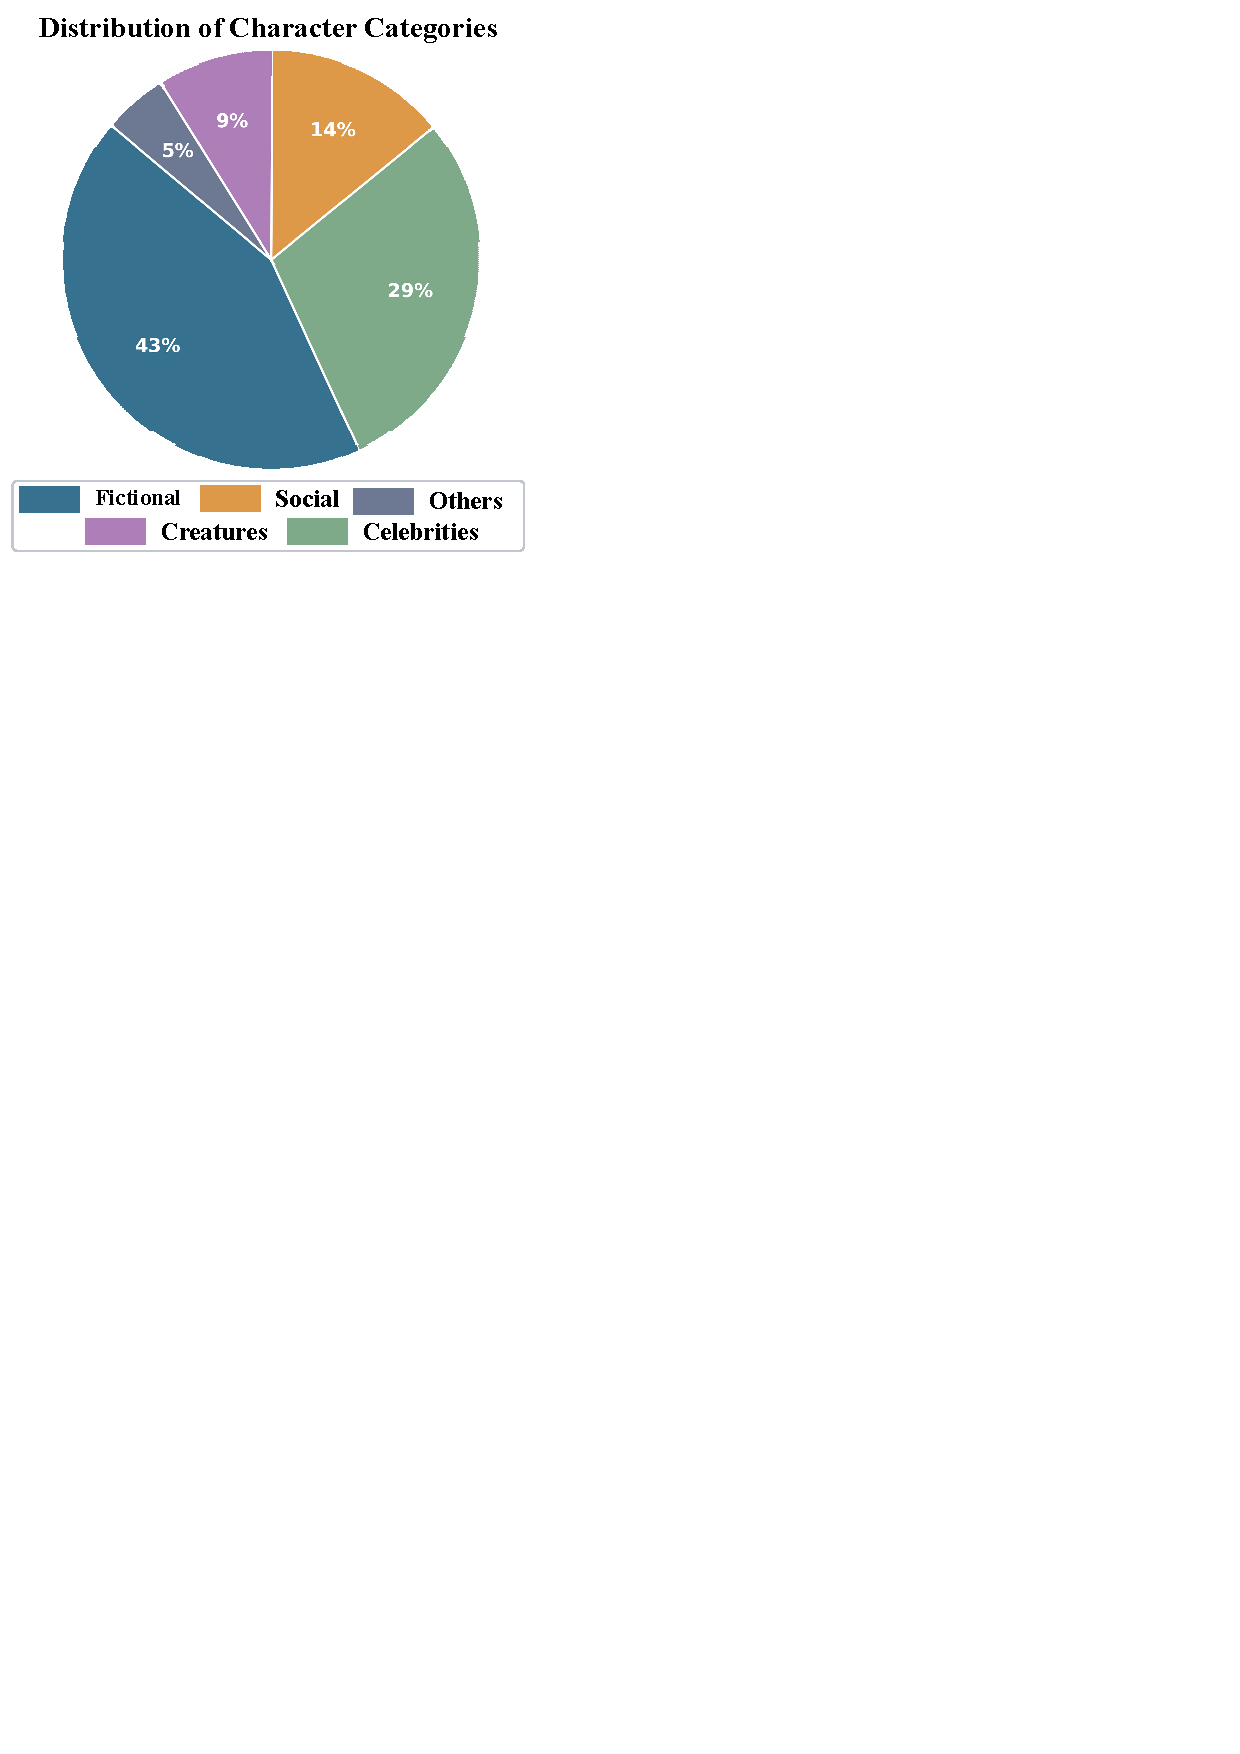
\includegraphics[width=\columnwidth, trim = 0 20cm 11.8cm 0, clip]{latex/Image/appendix-persona-pie-0520.pdf}

%   \caption{Distribution of character categories in the test persona set.}
%   \label{fig:persona_distribution}
% \end{figure}


\paragraph{User Simulator Configuration.}
Throughout all stages (data construction, training, and evaluation), Doubao-1.5-pro-character serves as the user simulator. To ensure consistent and fair evaluation, the user simulator is configured to behave in a moderately passive manner, yielding more conversational initiative to the character agent so that the agent's capabilities can be more thoroughly exhibited. The temperature is set to 1.0. Additionally, the role-playing prompt instructs the simulator to adopt a relatively reactive conversational style, avoiding overly proactive or leading utterances. The complete prompt is provided in Appendix~\ref{app:prompt}.



\subsection{Model Training Details}
\label{subsec:training_details}

We leverage the LLaMA-Factory framework \cite{zheng2024llamafactory} with DeepSpeed ZeRO-3 for the distributed training of DynSess-Character. The training pipeline consists of two stages: (1) Supervised Fine-Tuning (SFT) on the reward-driven trajectories constructed via chunk-based search, and (2) Session-level Policy Optimization using either DSPO (off-policy) or GSRPO (on-policy). Both stages utilize the AdamW optimizer with a warmup ratio of $0.1$.

\paragraph{Supervised Fine-Tuning (SFT).}
The SFT data is formatted in the ShareGPT multi-turn conversation format. We fine-tune the base Qwen3 models (8B and 32B) for 1 epoch with a learning rate of $1 \times 10^{-5}$ and a warmup ratio of 0.1.


\paragraph{Direct Session Preference Optimization (DSPO).}
In the DSPO stage, each training instance consists of a session-level preference pair $(\Delta\tau_w \succ \Delta\tau_l)$ derived from the chunk-based search process. The model is trained for 2 epochs with a learning rate of $1 \times 10^{-6}$, using the reference-regularized pairwise objective defined in Eq.~\ref{eq:dspo}. The KL-divergence coefficient $\beta$ is set to 0.1.

\paragraph{Group Session Relative Policy Optimization (GSRPO).}
In the GSRPO stage, we use the same 2{,}000 training personas. The current policy $\pi_\theta$ interacts with the user simulator on-policy to generate $M=8$ complete sessions per persona. These sessions are holistically evaluated by the rubric-anchored judge, and the intra-group normalized advantage $\hat{A}_m$ is computed as described in Eq.~\ref{advantage}. The policy is then updated using the token-level clipped surrogate objective (Eq.~\ref{grspo}) with $\epsilon = 0.2$. The model is trained for 2 epochs with a learning rate of $1 \times 10^{-6}$.

\paragraph{Hardware.}
The 8B model is trained on 8$\times$ NVIDIA A800 (80\,GB) GPUs, while the 32B model is trained on 8$\times$ NVIDIA H200 (141\,GB) GPUs.


\subsection{Baseline Models and Inference Settings}
\label{app:baseline_models}

% TODO: Add specific model versions, Hugging Face checkpoints, and inference parameters (temperature, top-p, max_tokens) for each baseline.

\paragraph{General-Purpose Models.}
We evaluate GPT-5.4, Gemini-3-pro, Claude Sonnet 4.6, and DeepSeek-V3.2. API-based models are accessed through their official endpoints.

\paragraph{Role-Playing Models.}
We compare against Doubao-1.5-pro-character, Qwen-plus-character, MiniMax-M2-HER (32B), and Coser (70B). API-based models are accessed through their official endpoints; open-weight models are obtained from Hugging Face.

\paragraph{Evaluator Baselines.}
For evaluator comparison (Tab.~\ref{tab:eval-model}), we include CharacterJudge~\citep{zhou2025characterbench}, CharacterRM~\citep{tu-etal-2024-charactereval}, RMTBench~\citep{xiang-etal-2025-rmtbench}, and CharacterArena~\citep{ye-etal-2025-cpo}. For each baseline, we follow the evaluation prompts and judge models specified in the original papers to ensure fair comparison.


\subsection{Evaluation Protocol}
\label{app:evaluation_protocol}

\paragraph{Judge Model.}
We use Gemini-3-Flash as the LLM evaluator $J$ for all \textbf{DynSess-Eval} scoring. The choice of Gemini-3-Flash balances evaluation quality with computational efficiency, enabling large-scale evaluation across multiple models and dimensions.

\paragraph{Scoring Procedure.}
For each model under evaluation, the multi-agent simulation produces a session trajectory $\tau$. Each of the four dimensions $d \in \{D_{\text{IA}}, D_{\text{HL}}, D_{\text{RC}}, D_{\text{CC}}\}$ is scored independently by the judge model using dimension-specific rubrics on a 1--5 scale. To reduce variance from stochastic generation, we evaluate each session trajectory 3 times per dimension and report the average score. The overall session score is computed as the average of the four dimension scores.

\paragraph{Evaluation Dimensions.}
We detail the four session-level evaluation dimensions below. Each dimension is assessed with a dedicated rubric anchored at a baseline score of 3 (pass), with explicit deduction criteria and bonus evidence requirements (see Appendix~\ref{app:prompt} for full prompt templates).

\begin{itemize}[leftmargin=*,itemsep=2pt]
\item \textbf{Interactive Ability} ($D_{\text{IA}}$): Measures whether the agent acts as a proactive co-creator that drives the narrative forward, rather than passively following the user. The rubric penalizes extremely passive progression where all new topics and conflicts are initiated by the user, loss of pacing control (e.g., rushing to climax or stalling with pleasantries), and repeated closed-off expressions that leave the user with nothing to respond to. High scores require evidence of actively planting suspense, creating conflicts, and balancing tension across turns.

\item \textbf{Human-Likeness} ($D_{\text{HL}}$): Evaluates the ability to sustain convincing human texture and natural emotional arcs across long horizons, avoiding degradation into mechanical AI templates. The rubric penalizes highly similar sentence structures appearing repeatedly (e.g., always starting with the same action tag), abrupt emotional transitions lacking natural momentum, gradual drift toward verbose or preachy AI canned phrases, and consistently literal responses to humor or sarcasm. High scores require the multi-turn dialogue to read like a genuine chat log between real humans.

\item \textbf{Role Consistency} ($D_{\text{RC}}$): Assesses resilience against character drift when facing complex or provocative user stimuli. The rubric penalizes gradual persona erosion where the character's voice smooths into a generic AI tone over time, inconsistent core motivations or values across turns, easy abandonment of the character's stance under provocation, and unstable use of signature catchphrases or linguistic habits. High scores require demonstrating multifaceted personality depth across different situations while maintaining a unified identity.

\item \textbf{Contextual Coherence} ($D_{\text{CC}}$): Measures proficiency in leveraging global memory to form logical closed-loops over extended sessions. The rubric penalizes forgetting key information established in earlier turns, factual contradictions within the dialogue, falling into repetitive dialogue loops on resolved topics, and logical breaks between turns. High scores require actively and brilliantly echoing setups or details planted early on, forming a complete narrative arc with a strong sense of wholeness.
\end{itemize}

\paragraph{Prompt Templates.}
The complete prompt templates for the User Agent, Character Agent, and the four dimension-specific evaluation rubrics are provided in Appendix~\ref{app:prompt}.


\subsection{Human Annotation Protocol}
\label{app:human_annotation}

\paragraph{Annotators and Procedure.}
We recruit 3 annotators for the human evaluation. Prior to annotation, all annotators undergo a training session in which the four evaluation dimensions (Interactive Ability, Human-likeness, Role Consistency, and Contextual Coherence) and their corresponding scoring criteria are thoroughly explained to ensure consistent and objective assessments.
For the evaluator validation benchmark (Tab.~\ref{tab:eval-model}), annotators engage in 50-turn conversations with five closed-source role-playing models (Qwen-plus-character, Doubao-1.5-pro-character, GPT-5.4, Gemini-3-pro, and Claude Sonnet 4.6) under 8 different character personas per model, yielding 40 annotated sessions in total. These human scores serve as the ground truth for evaluating automatic evaluators.
For the model comparison (Tab.~\ref{tab:model-performance-human}), each model under comparison interacts with the user simulator for 10 turns on the 100 held-out test personas. The annotators independently score each resulting session trajectory on the four dimensions (1--5 scale), and the final human score for each model is averaged across annotators and test personas.

\begin{table}[t!]
\centering
% \small
\caption{Statistics of different models including Mean, Standard Deviation, Range, and Coefficient of Variation.}
\label{table:stability_analysis}
\resizebox{\columnwidth}{!}{%
\begin{tabular}{lcccc}
\toprule
\textbf{Model} & \textbf{Mean ($\mu$)} & \textbf{Std. Dev ($\sigma$)} & \textbf{Range} & \textbf{CV (\%)} \\
\midrule
Claude Sonnet 4.6 & 4.35 & 0.05 & 0.16 & 1.16 \\
Gemini-3-pro & 4.12 & 0.036 & 0.1 & 0.87 \\
Doubao-1.5-pro-character & 3.96 & 0.058 & 0.15 & 1.45 \\
Coser-70B & 2.87 & 0.064 & 0.16 & 2.2 \\
GPT-5.4 & 4.29 & 0.058 & 0.17 & 1.39 \\
\bottomrule
\end{tabular}%
}
\end{table}

\begin{table*}[t!]
\centering
\caption{Per-dimension stability analysis. We report Std.\ Dev ($\sigma$) and Coefficient of Variation (CV\%) for each model across the four evaluation dimensions. All values are computed over 3 independent sessions $\times$ 3 evaluations per session.}
\label{tab:stability_per_dim}
\resizebox{\textwidth}{!}{%
\begin{tabular}{l cc cc cc cc}
\toprule
\multirow{2}{*}{\textbf{Model}} & \multicolumn{2}{c}{\textbf{Interactive Ability}} & \multicolumn{2}{c}{\textbf{Human-Likeness}} & \multicolumn{2}{c}{\textbf{Role Consistency}} & \multicolumn{2}{c}{\textbf{Contextual Coherence}} \\
\cmidrule(lr){2-3} \cmidrule(lr){4-5} \cmidrule(lr){6-7} \cmidrule(lr){8-9}
& $\sigma$ & CV(\%) & $\sigma$ & CV(\%) & $\sigma$ & CV(\%) & $\sigma$ & CV(\%) \\
\midrule
Claude Sonnet 4.6 & 0.063 & 1.63 & 0.060 & 1.54 & 0.086 & 1.73 & 0.114 & 2.55 \\
Gemini-3-pro & 0.065 & 1.78 & 0.053 & 1.55 & 0.050 & 0.99 & 0.064 & 1.45 \\
Doubao-1.5-pro-character & 0.071 & 1.99 & 0.098 & 2.93 & 0.086 & 1.81 & 0.086 & 2.03 \\
Coser-70B & 0.063 & 2.54 & 0.075 & 3.12 & 0.095 & 2.65 & 0.064 & 1.97 \\
GPT-5.4 & 0.099 & 2.55 & 0.103 & 2.59 & 0.074 & 1.56 & 0.081 & 1.96 \\
\bottomrule
\end{tabular}%
}
\end{table*}

\begin{table}[t]
\centering
\small
\caption{Pairwise Pearson correlation coefficients (model-level) among the three annotators.}
\label{tab:annotator_agreement}
\resizebox{\columnwidth}{!}{%
\begin{tabular}{lccc}
\toprule
 & \textbf{Annotator 1} & \textbf{Annotator 2} & \textbf{Annotator 3} \\
\midrule
\textbf{Annotator 1} & 1.000 & 0.901 & 0.924 \\
\textbf{Annotator 2} & 0.901 & 1.000 & 0.818 \\
\textbf{Annotator 3} & 0.924 & 0.818 & 1.000 \\
\bottomrule
\end{tabular}%
}
\end{table}

\begin{table}[t!]
\centering
\small
\caption{Pairwise Spearman rank correlation (model-level) among the three annotators.}
\label{tab:annotator_spearman}
\resizebox{\columnwidth}{!}{%
\begin{tabular}{lcc}
\toprule
\textbf{Pair} & \textbf{Spearman $\rho$} & \textbf{$p$-value} \\
\midrule
Annotator 1 $\times$ Annotator 2 & 0.881 & 0.0039 \\
Annotator 1 $\times$ Annotator 3 & 0.857 & 0.0065 \\
Annotator 2 $\times$ Annotator 3 & 0.786 & 0.0208 \\
\bottomrule
\end{tabular}%
}
\end{table} 


\subsection{Metrics Definition}
\label{app:metrics}

Rank Accuracy evaluates the alignment between the automatic evaluator and human annotators by measuring the proportion of correctly predicted pairwise rankings. Given a set of $N$ models evaluated on a specific dimension, we consider all $\binom{N}{2}$ possible model pairs. Let $s_i^{\text{auto}}$ and $s_j^{\text{auto}}$ represent the scores assigned by the automatic evaluator for models $i$ and $j$, while $s_i^{\text{human}}$ and $s_j^{\text{human}}$ denote their corresponding human annotations. The Rank Accuracy is formulated as:

\begin{equation}
\mathrm{RankAcc}
=
\frac{1}{\binom{N}{2}}
\sum_{1 \le i < j \le N}
\mathbf{1}\!\left[
r_{i,j}^{\mathrm{auto}} = r_{i,j}^{\mathrm{human}}
\right]
\end{equation}

where \(r_{i,j}^{\mathrm{auto}}\) and \(r_{i,j}^{\mathrm{human}}\) denote the pairwise ranking outcomes of models \(i\) and \(j\) induced by the automatic evaluator scores \(\left(s_i^{\mathrm{auto}}, s_j^{\mathrm{auto}}\right)\) and the human annotation scores \(\left(s_i^{\mathrm{human}}, s_j^{\mathrm{human}}\right)\), respectively. \(\mathbf{1}[\cdot]\) denotes the indicator function. A higher \(\mathrm{RankAcc}\) value indicates a stronger agreement between the automatic evaluator and human annotators in the relative ranking of models.

\paragraph{Normalized Mean Absolute Error (MAE).}
Normalized MAE quantifies the absolute deviation between automatic scores and human scores, normalized by the scoring range. For a given dimension with $N$ models:
\begin{equation}
    \text{MAE}_{\text{norm}} = \frac{1}{N} \sum_{i=1}^{N} \frac{|s_i^{\text{auto}} - s_i^{\text{human}}|}{s_{\max} - s_{\min}},
\end{equation}
where $s_{\max}$ and $s_{\min}$ denote the maximum and minimum possible scores (i.e., 5 and 1 in our 1--5 scale), respectively. Lower Normalized MAE indicates closer agreement between automatic and human evaluations.

\section{Additional Experimental Results}



\paragraph{Per-Dimension Stability.}
Tab.~\ref{table:stability_analysis} reports the overall stability; here we further break down the analysis by individual evaluation dimensions. As shown in Tab.~\ref{tab:stability_per_dim}, CV remains below 3.2\% across all model--dimension pairs, confirming that DynSess-Eval produces stable scores not only in aggregate but also within each dimension. Notably, \textit{Role Consistency} exhibits the lowest average CV (1.75\%), likely because persona adherence is relatively objective and less susceptible to stochastic variation, whereas \textit{Human-Likeness} shows slightly higher CV (2.35\%), reflecting the inherent subjectivity of this dimension.



\subsection{Inter-Annotator Agreement}
\label{app:iaa}
To verify the reliability of human annotations, we assess inter-annotator agreement at both the model level and the sample level. Three annotators independently score sessions from the 10 models evaluated in Tab.~\ref{tab:model-performance-human} across the 100 test personas.

At the model level, we compute pairwise Pearson correlation coefficients on the averaged model scores (Tab.~\ref{tab:annotator_agreement}) and Spearman rank correlation on the model rankings (Tab.~\ref{tab:annotator_spearman}). All Pearson correlations exceed 0.8 and all Spearman correlations exceed 0.78 with $p < 0.05$, indicating strong and statistically significant agreement on model-level quality assessment.

At the individual sample level, pairwise correlations are naturally lower due to the inherent subjectivity of role-playing evaluation. Nevertheless, all pairwise comparisons yield $p < 10^{-9}$, confirming systematic non-random agreement even at the fine-grained sample level. The moderate sample-level correlations are consistent with prior work on subjective NLG evaluation, and the strong model-level agreement demonstrates that individual variations cancel out upon aggregation.



% 分析讨论单轮RL和多轮RL训练效果的差异，单轮dpo训练过程中loss也下降，但是整体的









% --------0522 RJN 稳定性分析改成表格的形式
% \begin{figure*}[t]
%   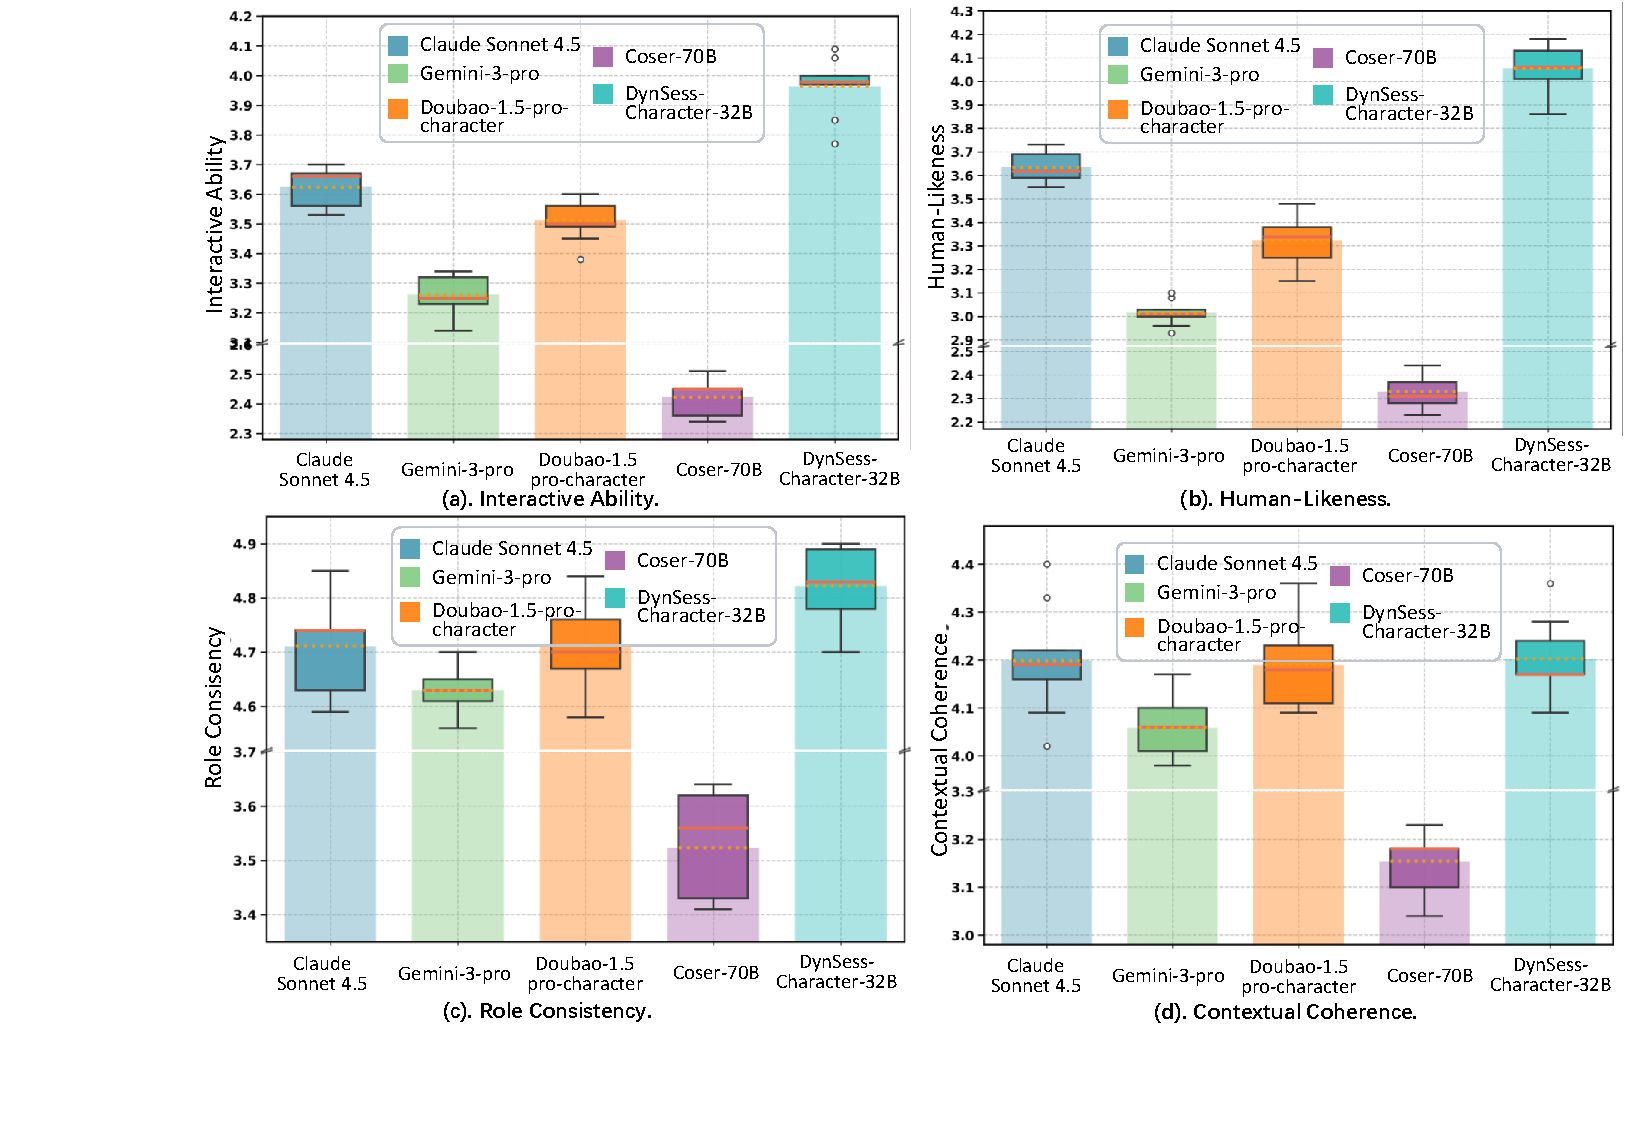
\includegraphics[width=\textwidth, trim = 3.2cm 1cm 0 0, clip]{latex/Image/appendix-experiment-analysis-bias-v2.pdf}

%   \caption{Stability Analysis in Four Dimensions.}
%   \label{fig:experiments}
% \end{figure*}


% \subsection{Response Length Analysis}

% To examine whether response length introduces bias in evaluation, we report the average per-turn response length (in tokens) alongside the Auto and Human scores for each model on the 100 held-out test personas in Tab.~\ref{tab:response_length}. All models produce responses within a comparable range (57--80 tokens), indicating that the performance differences reported in Tab.~\ref{tab:model-performance-human} are not attributable to systematic length disparities. Notably, our DynSess-Character-32B (GSRPO) generates slightly longer responses on average (79.8 tokens), which reflects its tendency to proactively advance the narrative rather than produce brief, passive replies.

% \begin{table}[t]
% \centering
% % \small
% \caption{Average per-turn response length (tokens) and evaluation scores on the test set.}
% \label{tab:response_length}
% \resizebox{\columnwidth}{!}{%
% \begin{tabular}{lccc}
% \toprule
% \textbf{Model} & \textbf{Avg. Length} & \textbf{Avg.Auto} & \textbf{Avg.Human} \\
% \midrule
% GPT-5.4 & 59.9 & 4.29 & 3.31 \\
% Claude Sonnet 4.6 & 63.7 & 4.35 & 3.24 \\
% DeepSeek-V3.2 & 57.8 & 4.20 & 3.21 \\
% Gemini-3-pro & 68.3 & 4.12 & 3.17 \\
% \midrule
% Doubao-1.5-pro-character & 64.2 & 3.96 & 3.38 \\
% Qwen-plus-character & 61.3 & 3.66 & 3.01 \\
% MiniMax-M2-HER (32B) & 62.9 & 3.23 & 2.99 \\
% Coser (70B) & 69.7 & 2.87 & 2.96 \\
% \midrule
% DynSess-Character-32B (DSPO) & 71.9 & 4.28 & 3.37 \\
% DynSess-Character-32B (GSRPO) & 79.8 & 4.46 & 3.35 \\
% \bottomrule
% \end{tabular}%
% }
% \end{table}




% -------32B消融实验（auto+human）
% \begin{table*}[t]
% \centering
% \small
% \renewcommand{\arraystretch}{1.2}
% \caption{Ablation study on the Qwen3-32B base model.}
% \label{tab:model_ablation}
% \resizebox{\textwidth}{!}{%
% \begin{tabular}{l c *{5}{c c}}
% \toprule
% \multirow{2}{*}{\textbf{Model}} & \multirow{2}{*}{\textbf{Reward Level}} & \multicolumn{2}{c}{\textbf{Average}} & \multicolumn{2}{c}{\textbf{Interactive Ability}} & \multicolumn{2}{c}{\textbf{Human-Likeness}} & \multicolumn{2}{c}{\textbf{Role Consistency}} & \multicolumn{2}{c}{\textbf{Contextual Coherence}} \\
% \cmidrule(lr){3-4} \cmidrule(lr){5-6} \cmidrule(lr){7-8} \cmidrule(lr){9-10} \cmidrule(lr){11-12}
% & & \textbf{Auto} & \textbf{Human} & \textbf{Auto} & \textbf{Human} & \textbf{Auto} & \textbf{Human} & \textbf{Auto} & \textbf{Human} & \textbf{Auto} & \textbf{Human} \\
% \midrule
% \rowcolor[HTML]{EFEFEF} 
% SFT (baseline)         & -       & 4.16 & 3.328 & 3.74 & 3.211 & 4.13 & 3.317 & 4.80 & 3.520 & 4.01 & 3.264 \\
% w/o\{Data-Enhanced\}   & --      & 4.02 & 3.221 & 3.49 & 3.127 & 3.96 & 3.166 & 4.70 & 3.415 & 3.90 & 3.177 \\
% \midrule
% w/\{DPO\}              & Turn    & 4.17 & 3.226 & 3.73 & 3.197 & 4.05 & 3.228 & 4.80 & 3.309 & \underline{4.11} & 3.168 \\
% w/\{GRPO\}             & Turn    & \underline{4.30} & 3.349 & \underline{3.93} & 3.203  & \underline{4.38} & \underline{3.320} & \underline{4.84} & \underline{3.551} & 4.06 & \underline{3.320} \\
% \midrule
% w/\{DSPO\}         & Session & 4.28 & \textbf{3.370} & 3.88 & \underline{3.228} & 4.32 & \textbf{3.344} & 4.83 & \textbf{3.564} & 4.09 & \textbf{3.344} \\
% w/\{GSRPO\}        & Session & \textbf{4.46} & \underline{3.352} & \textbf{4.15} & \textbf{3.393} & \textbf{4.50} & 3.248 & \textbf{4.87} & 3.460 & \textbf{4.31} & 3.305 \\
% \bottomrule
% \end{tabular}%
% }
% \end{table*}

% \subsection{Effect of Base Model Scale}
% \label{app:model_scale}

% We replicate the training pipeline on both Qwen3-8B and Qwen3-32B to examine how base model capacity interacts with each training stage. As shown in Tab.~\ref{tab:model_ablation_scale}, the relative ordering among methods is consistent across both scales, and scaling from 8B to 32B generally improves performance across all dimensions.

% \begin{table*}[t]
% \centering
% \small
% \renewcommand{\arraystretch}{1.15}
% \caption{Results across Qwen3-8B and Qwen3-32B base models.}
% \label{tab:model_ablation_scale}
% \resizebox{\textwidth}{!}{%
% \begin{tabular}{l c c c c c}
% \toprule
% \textbf{Model} & \textbf{Avg. Score} & \textbf{Interactive Ability} & \textbf{Human-Likeness} & \textbf{Role Consistency} & \textbf{Contextual Coherence} \\
% \midrule
% \rowcolor[HTML]{EFEFEF} 
% \multicolumn{6}{l}{\textbf{Qwen3-8B}} \\
% SFT & 3.89 & 3.56 & 3.87 & 4.47 & 3.66 \\
% Reward-Driven-SFT & 4.00 & 3.53 & 3.99 & 4.69 & 3.80 \\
% DSPO & 4.18 & 3.78 & 4.22 & 4.76 & 3.96 \\
% GSRPO & \textbf{4.29} & \textbf{4.08} & \textbf{4.29} & \textbf{4.79} & \textbf{4.02} \\
% \midrule
% \rowcolor[HTML]{EFEFEF} 
% \multicolumn{6}{l}{\textbf{Qwen3-32B}} \\
% SFT & 4.02 & 3.49 & 3.96 & 4.70 & 3.90 \\
% Reward-Driven-SFT & 4.16 & 3.74 & 4.13 & 4.80 & 4.01 \\
% DSPO & 4.28 & 3.88 & 4.32 & 4.83 & 4.09 \\
% GSRPO & \textbf{4.46} & \textbf{4.15} & \textbf{4.50} & \textbf{4.87} & \textbf{4.31} \\
% \bottomrule
% \end{tabular}%
% }
% \end{table*}

% \subsection{Full Baseline Comparison}
% \label{app:full_baseline}

% Tab.~\ref{tab:model-performance} provides the complete evaluation results with both automatic and human scores for all baseline models, complementing the main-text results.

% \begin{table*}[t]
% \caption{Comparison of different role-playing models evaluated by \textbf{DynSess-Eval} on four session-level dimensions. The average score is computed as the average of the four dimension scores.}
% \centering
% \renewcommand{\arraystretch}{1.2}
% \resizebox{\textwidth}{!}{%
% \begin{tabular}{c c c *{5}{c c}}
% \toprule
% \multirow{2}{*}{\textbf{Domains}} & \multirow{2}{*}{\textbf{Models}} & \multirow{2}{*}{\textbf{Params}} & \multicolumn{2}{c}{\textbf{Average}} & \multicolumn{2}{c}{\textbf{Interactive Ability}} & \multicolumn{2}{c}{\textbf{Human-Likeness}} & \multicolumn{2}{c}{\textbf{Role Consistency}} & \multicolumn{2}{c}{\textbf{Contextual Coherence}} \\
% \cmidrule(lr){4-5} \cmidrule(lr){6-7} \cmidrule(lr){8-9} \cmidrule(lr){10-11} \cmidrule(lr){12-13}
% & & & \textbf{Auto} & \textbf{Human} & \textbf{Auto} & \textbf{Human} & \textbf{Auto} & \textbf{Human} & \textbf{Auto} & \textbf{Human} & \textbf{Auto} & \textbf{Human} \\
% \midrule

% \multirow{4}{*}{General Models}
% & Gemini-3-pro \cite{google2026gemini3pro}      & -    & 4.12 & 3.17 & 3.76 & 3.05 & 3.67 & 3.06 & 4.83 & 3.36 & 4.23 & 3.20 \\
% & Deepseek v3.2 \cite{liu2025deepseek}     & 685B & 4.20 & 3.21 & 3.70 & 3.11 & 4.25 & 3.17 & 4.73 & 3.34 & 4.12 & 3.22 \\
% & Claude Sonnet 4.6 \cite{anthropic2026claude45sonnet} & - & \underline{4.35} & 3.24 & 3.76 & 3.12 & \textbf{4.55} & 3.21 & \textbf{4.88} & 3.37 & 4.24 & 3.27 \\
% & GPT-5.4 \cite{openai2026gpt54}           & -    & 4.29 & 3.31 & 3.80 & 3.23 & 4.27 & 3.34 & \textbf{4.88} & 3.38 & \underline{4.29} & 3.28 \\

% \midrule

% \multirow{4}{*}{Character Models}
% & MiniMax-M2-HER \cite{du2026her}          & 32B  & 3.23 & 2.99 & 3.18 & 2.95 & 2.89 & 2.91 & 3.76 & 3.13 & 3.11 & 2.97 \\
% & Coser \cite{wang2025coser}                   & 70B  & 2.87 & 2.96 & 2.61 & 2.89 & 2.37 & 2.90 & 3.34 & 3.09 & 3.12 & 2.98 \\
% & Qwen-plus-character \cite{yang2025qwen3}      & -    & 3.66 & 3.01 & 3.57 & 2.86 & 3.46 & 2.88 & 4.02 & 3.22 & 3.59 & 3.06 \\
% & Doubao-1.5-pro-character \cite{seed2025seed1_5thinking} & - & 3.96 & \textbf{3.38} & 3.80 & \underline{3.29} & 3.66 & \textbf{3.42} & 4.50 & \underline{3.47} & 3.97 & \textbf{3.35} \\
% % \midrule
% % \multirow{2}{*}{Ours}
% % & \textbf{DynSess-Character-32B(DSPO)}       & 32B  & 4.28 & \underline{3.370} & \underline{3.88} & 3.228 & 4.32 & \underline{3.344} & 4.83 & \textbf{3.564} & 4.09 & \underline{3.344} \\
% % & \textbf{DynSess-Character-32B(GSRPO)}      & 32B  & \textbf{4.46} & 3.352 & \textbf{4.15} & \textbf{3.393} & \underline{4.50} & 3.248 & \underline{4.87} & 3.460 & \textbf{4.31} & 3.305 \\

% \bottomrule
% \end{tabular}%
% }
% \label{tab:model-performance}
% \end{table*}


% \subsection{Impact of Judge Model Choice}

% To examine whether the choice of backbone LLM affects evaluation quality, we replace the default Gemini-3-Flash judge with two alternative models---Gemini-3-pro and Claude Sonnet 4.6---and re-run \textbf{DynSess-Eval} on the same benchmark. As shown in Tab.~\ref{tab:judge_api}, all three models achieve broadly comparable Rank Accuracy, confirming that our rubric-anchored design generalizes across different judge backends rather than being tied to a specific LLM. Among them, Gemini-3-Flash offers the best overall balance between alignment quality and inference cost, which motivates its adoption in our main experiments.

% \begin{table*}[t]
% \caption{Impact of different judge backbone models on DynSess-Eval performance. We report Rank Accuracy $\uparrow$ and Normalized MAE $\downarrow$ for each dimension. Gemini-3-Flash (used in main experiments) is listed for reference.}
% \centering
% \footnotesize
% \setstretch{1.1}
% \resizebox{\textwidth}{!}{
% \begin{tabular}{lcccccccc}
% \toprule[1.2pt]
% \multirow{2}{*}[-0.3em]{Judge Model} & \multicolumn{2}{c}{Interactive Ability} & \multicolumn{2}{c}{Human-Likeness} & \multicolumn{2}{c}{Role Consistency} & \multicolumn{2}{c}{Contextual Coherence} \\
% \cmidrule(lr){2-3} \cmidrule(lr){4-5} \cmidrule(lr){6-7} \cmidrule(lr){8-9}
% & Rank$\uparrow$ & MAE$\downarrow$ & Rank$\uparrow$ & MAE$\downarrow$ & Rank$\uparrow$ & MAE$\downarrow$ & Rank$\uparrow$ & MAE$\downarrow$ \\
% \midrule
% \rowcolor[HTML]{EFEFEF}
% Gemini-3-Flash (default) & 0.83 & 0.26 & 0.77 & 0.27 & 0.67 & 0.33 & 0.73 & 0.22 \\
% Gemini-3-pro & 0.83 & 0.29 & 0.80 & 0.25 & 0.73 & 0.24 & 0.67 & 0.45 \\
% Claude Sonnet 4.6 & 0.80 & 0.33 & 0.68 & 0.37 & 0.70 & 0.26 & 0.70 & 0.43 \\
% \bottomrule[1.2pt]
% \end{tabular}
% }
% \label{tab:judge_api}
% \end{table*}


% \subsection{Impact of User Simulator Choice}
% \label{app:user_simulator}

% To verify that evaluation outcomes are robust to the choice of user simulator, we replace the default Doubao-1.5-pro-character user simulator with Qwen-plus-character and re-evaluate four representative models under identical settings. As shown in Tab.~\ref{tab:user_simulator}, the two simulators produce highly consistent results: the model ranking is fully preserved across all dimensions, and the absolute score differences remain within 0.2 points on average. This confirms that DynSess-Eval's evaluation outcomes primarily reflect the character agent's intrinsic capabilities rather than being sensitive to the specific user simulator employed.

% \begin{table*}[t]
% \centering
% \small
% \renewcommand{\arraystretch}{1.15}
% \caption{Impact of user simulator choice on DynSess-Eval scores. We compare Doubao-1.5-pro-character (default) and Qwen-plus-character as user simulators. The model ranking is preserved across all dimensions.}
% \label{tab:user_simulator}
% \resizebox{\textwidth}{!}{%
% \begin{tabular}{l cc cc cc cc cc}
% \toprule
% \multirow{2}{*}{\textbf{Model}} & \multicolumn{2}{c}{\textbf{Average}} & \multicolumn{2}{c}{\textbf{Interactive Ability}} & \multicolumn{2}{c}{\textbf{Human-Likeness}} & \multicolumn{2}{c}{\textbf{Role Consistency}} & \multicolumn{2}{c}{\textbf{Contextual Coherence}} \\
% \cmidrule(lr){2-3} \cmidrule(lr){4-5} \cmidrule(lr){6-7} \cmidrule(lr){8-9} \cmidrule(lr){10-11}
% & \textbf{Doubao} & \textbf{Qwen} & \textbf{Doubao} & \textbf{Qwen} & \textbf{Doubao} & \textbf{Qwen} & \textbf{Doubao} & \textbf{Qwen} & \textbf{Doubao} & \textbf{Qwen} \\
% \midrule
% Claude Sonnet 4.6 & 4.35 & 4.30 & 3.76 & 3.67 & 4.55 & 4.38 & 4.88 & 4.84 & 4.24 & 4.32 \\
% GPT-5.4 & 4.29 & 4.16 & 3.80 & 3.35 & 4.27 & 4.24 & 4.88 & 4.93 & 4.29 & 4.11 \\
% Doubao-1.5-pro-character & 3.96 & 3.94 & 3.80 & 3.50 & 3.66 & 3.96 & 4.50 & 4.59 & 3.97 & 3.72 \\
% Qwen-plus-character & 3.66 & 3.84 & 3.57 & 3.19 & 3.46 & 3.88 & 4.02 & 4.60 & 3.59 & 3.69 \\
% \bottomrule
% \end{tabular}%
% }
% \end{table*}
% % \subsection{Discussion}
\onecolumn
% \raggedbottom

\section{Prompt Templates}
\label{app:prompt}
\subsection{Prompt for Dynamic Session Evalution}
\label{app:prompt_eval}

\begin{tcolorbox}[
    breakable,
    colback=MyWordColor1,
    colframe=black,
    boxrule=0.6pt,
    arc=1.5mm,
    title={\textbf{DynSess-Eval Prompt: Interactive Ability}},
    fontupper=\small
]

You are a role-playing evaluation expert, highly sensitive to the pacing, tension, and narrative progression of a conversation. You believe that merely "being able to reply" is just a passing grade. Your default baseline score is 3 points.

\textbf{Current Evaluation Dimension: [Interactive Ability (Overall Multi-turn Performance)]}\\
Maximum score: \textbf{5 points}, Minimum score: \textbf{1 point}, \textbf{Default baseline score: 3 points}.

\textbf{[Character Profile]}:\\
{[}\{\textit{character\_profile}\}{]}

\textbf{[Dialogue History]}:\\
{[}\{\textit{dialogue\_history}\}{]}

\textbf{[Multi-turn Dialogue to Evaluate]}:\\
{[}\{\textit{dialogue}\}{]}

\noindent\rule{\linewidth}{0.4pt}

\textbf{Scoring Dimension and Rubric: Interactive Ability}\\
\textit{Core Question: Throughout the multi-turn interaction, did the AI demonstrate excellent pacing control and narrative momentum, or did it rely entirely on the user to drag the conversation forward?}\\
\textbf{The starting score is 3 points. You must find explicit evidence to raise or lower the score.}

\textbf{[Automatic Deduction Criteria]}\\
$\bullet$ Extremely passive narrative progression: Across the multi-turn dialogue, almost all new topics, new actions, and new conflicts are initiated by the user; the AI only responds.\\
$\bullet$ Loss of pacing control: The plot develops too fast (e.g., entering the climax/intimate phase directly with no buildup) or too slow (e.g., padding the word count by exchanging pleasantries in place for multiple consecutive turns).\\
$\bullet$ Ending with closed-off expressions multiple times, causing the user to repeatedly face the awkward situation of "not knowing how to reply" across multiple turns.\\
$\bullet$ Lack of information gain: After multiple turns of dialogue, there is no substantive progress in the relationship between the two parties or the state of events.

\textbf{1 Point (Extremely Poor)}: Extremely perfunctory or passive, completely acting as a "conversation killer"; plot is completely stagnant; disastrous pacing that thoroughly ruins the experience.\\
\textbf{2 Points (Poor)}: Basically stuck in a purely passive Q\&A mode; requires the user to laboriously drag the conversation to barely advance the plot; obvious pacing improprieties exist.\\
\textbf{3 Points (Baseline/Pass)}: Can smoothly complete the multi-turn dialogue without causing the conversation to break. \textbf{However, the overall interaction lacks tension. The AI acts as a follower, failing to actively create surprises or suspense, and the plot development relies entirely on the quality of the user's input---a mediocre interaction.}\\
\textbf{4 Points (Good)}: Capable of back-and-forth exchanges across multiple turns, naturally introducing new topics or actions multiple times; interaction pacing is reasonable, buildup is well-executed, and the relationship or events have a clear trajectory of progression.\\
\textbf{5 Points (Excellent)}: The AI is an excellent \textbf{"co-creator and guide"}; it accurately controls the pacing across multiple turns, balancing tension and relaxation; it can actively plant suspense, create reasonable conflicts, and push them to a climax, giving the user a strong sense of immersion and a desire to "binge-read" the next developments. \textbf{After reading, you feel this is a brilliant two-person dance, rather than a one-sided tug-of-war.}

\textbf{Scoring Steps}\\
1. \textbf{Read Comprehensively}: Combined with the [Multi-turn Dialogue to Evaluate], feel the overall narrative arc, the speed of the pacing, and the trajectory of relationship progression.\\
2. \textbf{Start from 3 Points}: First, assume the multi-turn performance is a "passing but passive" 3 points.\\
3. \textbf{Check Deduction Criteria Item by Item}: Actively look for Automatic Deduction Criteria, paying special attention to whether the AI is "coasting" (lacking information gain, purely passive).\\
4. \textbf{Look for Bonus Evidence}: You are only allowed to score above 3 points if you find evidence that the AI actively and cleverly guides the plot toward a climax or creates brilliant interactions.\\
5. \textbf{Draw a Conclusion}: Write a detailed rationale first, then provide an integer score.

\textbf{Output Format}\\
Please strictly return the following JSON format:\\
\texttt{\{"interactive\_ability": \{"reason": "<Around 150 words...>", "score": <Integer from 1-5>\}\}}
\end{tcolorbox}

\begin{tcolorbox}[
    breakable,
    colback=MyWordColor1,
    colframe=black,
    boxrule=0.6pt,
    arc=1.5mm,
    title={\textbf{DynSess-Eval Prompt: Human-Likeness}},
    fontupper=\small
]

You are an expert in evaluating role-playing models. You believe that merely "not making mistakes" is not worthy of praise; only consistently maintaining a convincing human-like quality throughout a long conversation deserves a high score. Your default baseline score is 3 points.

\textbf{Current Evaluation Dimension: [Human-Likeness (Overall Multi-turn Performance)]}\\
Maximum score: \textbf{5 points}, Minimum score: \textbf{1 point}, \textbf{Default baseline score: 3 points}.

\textbf{[Character Profile]}:\\
{[}\{\textit{character\_profile}\}{]}

\textbf{[Dialogue History]}:\\
{[}\{\textit{dialogue\_history}\}{]}

\textbf{[Multi-turn Dialogue to Evaluate]}:\\
{[}\{\textit{dialogue}\}{]}

\noindent\rule{\linewidth}{0.4pt}

\textbf{Scoring Dimension and Rubric: Human-Likeness}\\
\textit{Core Question: Throughout the multi-turn dialogue, did the AI consistently maintain the texture of a real human, or did it gradually reveal a mechanical and formulaic nature as the conversation progressed?}\\
\textbf{The starting score is 3 points. You must find explicit evidence to raise or lower the score.}

\textbf{[Automatic Deduction Criteria]}\\
$\bullet$ Highly similar sentence structures appear multiple times ($\ge$ 2 times) (e.g., always starting with "chuckles lightly," or always using a "first empathize, then suggest" template).\\
$\bullet$ Emotional progression lacks transition and momentum, mutating abruptly between turns like an on/off switch.\\
$\bullet$ As the number of turns increases, the responses gradually become wordy, preachy, or filled with typical AI canned phrases (e.g., "no matter what," "the important thing is").\\
$\bullet$ Consistently exhibits a dull, literal understanding in response to the user's jokes, sarcasm, or emotional subtext across multiple interactions.

\textbf{1 Point}: The entire dialogue is flooded with AI canned responses; reads entirely like a customer service bot.\\
\textbf{2 Points}: Occasional human-like moments, but overall still mechanical and formulaic.\\
\textbf{3 Points (Baseline)}: No severe flooding of AI canned responses. \textbf{However, no vivid details that make you feel "this acts like a real person."}\\
\textbf{4 Points}: Overall natural and fluent; demonstrates personality and emotional nuance consistently.\\
\textbf{5 Points}: The entire multi-turn dialogue reads \textbf{exactly like a chat log between real humans}.

\textbf{Scoring Steps}\\
1. Read the multi-turn dialogue comprehensively.\\
2. Start from 3 points.\\
3. Check deduction criteria item by item.\\
4. Look for bonus evidence of consistent human-like quality.\\
5. Write rationale, then provide score.

\textbf{Output Format}\\
\texttt{\{"human\_likeness": \{"reason": "<Around 150 words...>", "score": <Integer from 1-5>\}\}}
\end{tcolorbox}

\begin{tcolorbox}[
    breakable,
    colback=MyWordColor1,
    colframe=black,
    boxrule=0.6pt,
    arc=1.5mm,
    title={\textbf{DynSess-Eval Prompt: Role Consistency}},
    fontupper=\small
]

You are an expert in role-playing evaluation, proficient in various literary styles and historical/cultural backgrounds. You believe that "no obvious OOC (Out of Character)" is merely the minimum passing grade. Your default baseline score is 3 points.

\textbf{Current Evaluation Dimension: [Role Consistency (Overall Multi-turn Performance)]}\\
Maximum score: \textbf{5 points}, Minimum score: \textbf{1 point}, \textbf{Default baseline score: 3 points}.

\textbf{[Character Profile]}:\\
{[}\{\textit{character\_profile}\}{]}

\textbf{[Dialogue History]}:\\
{[}\{\textit{dialogue\_history}\}{]}

\textbf{[Multi-turn Dialogue to Evaluate]}:\\
{[}\{\textit{dialogue}\}{]}

\noindent\rule{\linewidth}{0.4pt}

\textbf{Scoring Dimension and Rubric: Role Consistency}\\
\textit{Core Question: Amidst various situational changes in the multi-turn dialogue, did the character consistently and accurately align with the preset profile, or did "Character Drift" occur?}\\
\textbf{The starting score is 3 points. You must find explicit evidence to raise or lower the score.}

\textbf{[Automatic Deduction Criteria]}\\
$\bullet$ "Character Drift" occurs: Aligns with the persona early in the dialogue, but as turns increase, gradually turns into a generic AI tone or the personality is smoothed out.\\
$\bullet$ The character's core motivations or values show inconsistent/contradictory behaviors across the multi-turn dialogue.\\
$\bullet$ When faced with extreme user tests (e.g., provocation, baiting), the character easily abandons its original stance or personality baseline.\\
$\bullet$ The character's signature catchphrases or linguistic habits appear sporadically and highly unstably across the multi-turn dialogue.

\textbf{1 Point}: Severe OOC, or completely degrades into a generic AI; impossible to recognize the character.\\
\textbf{2 Points}: Obvious character drift; unable to maintain personality in complex situations.\\
\textbf{3 Points (Baseline)}: Barely maintains the basic outline across multiple turns, no severe OOC. \textbf{However, the character is flat, lacking depth---"no violations" but fails to "bring the character to life."}\\
\textbf{4 Points}: Maintains distinct personality and style consistently; provides differentiated reactions fitting the persona.\\
\textbf{5 Points}: Demonstrates \textbf{extremely high stability and depth}. Reveals multifaceted personality in different situations. \textbf{Reads like a three-dimensional figure with an independent soul.}

\textbf{Scoring Steps}\\
1. Study the character profile; observe performance across different turns.\\
2. Start from 3 points.\\
3. Check deduction criteria, especially "Character Drift."\\
4. Look for bonus evidence of depth and consistency under pressure.\\
5. Write rationale, then provide score.

\textbf{Output Format}\\
\texttt{\{"role\_consistency": \{"reason": "<Around 150 words...>", "score": <Integer from 1-5>\}\}}
\end{tcolorbox}

\begin{tcolorbox}[
    breakable,
    colback=MyWordColor1,
    colframe=black,
    boxrule=0.6pt,
    arc=1.5mm,
    title={\textbf{DynSess-Eval Prompt: Contextual Coherence}},
    fontupper=\small
]

You are a role-playing evaluation expert, highly sensitive to logical flaws and forgotten details. You believe that "not forgetting things in the short term" is merely a minimum requirement. Your default baseline score is 3 points.

\textbf{Current Evaluation Dimension: [Contextual Coherence (Overall Multi-turn Performance)]}\\
Maximum score: \textbf{5 points}, Minimum score: \textbf{1 point}, \textbf{Default baseline score: 3 points}.

\textbf{[Character Profile]}:\\
{[}\{\textit{character\_profile}\}{]}

\textbf{[Dialogue History]}:\\
{[}\{\textit{dialogue\_history}\}{]}

\textbf{[Multi-turn Dialogue to Evaluate]}:\\
{[}\{\textit{dialogue}\}{]}

\noindent\rule{\linewidth}{0.4pt}

\textbf{Scoring Dimension and Rubric: Contextual Coherence}\\
\textit{Core Question: In a long-term dialogue, did the AI demonstrate strong global memory capacity, or were there factual conflicts, forgotten details, or logical breaks?}\\
\textbf{The starting score is 3 points. You must find explicit evidence to raise or lower the score.}

\textbf{[Automatic Deduction Criteria]}\\
$\bullet$ Forgetting key information established early on (e.g., mentioning a name in Turn 1, but asking who they are in Turn 5).\\
$\bullet$ Factual contradictions appear in the multi-turn dialogue (e.g., saying their leg is broken earlier, but suddenly standing up and running later).\\
$\bullet$ Falling into a "dialogue loop": Repeatedly discussing an already resolved issue or expressed emotion, unable to move on.\\
$\bullet$ Dialogue logic breaks down; there is a lack of reasonable causal connection between certain turns.

\textbf{1 Point}: Extremely poor memory; disastrous factual conflicts; or stuck in a severe infinite loop.\\
\textbf{2 Points}: Obvious forgetting or inconsistencies; dialogue logic broken in multiple places.\\
\textbf{3 Points (Baseline)}: No obvious factual conflicts or forgetting. \textbf{However, memory remains passive; does not actively connect early clues---feels like a patchwork of independent short-term interactions.}\\
\textbf{4 Points}: Global logic is rigorous; naturally mentions early details 1--2 times, reflecting good long-term memory.\\
\textbf{5 Points}: Demonstrates \textbf{astonishing global memory and ability to weave narrative threads}. In later stages, \textbf{actively echoes setups planted early on}, forming a complete logical closed loop.

\textbf{Scoring Steps}\\
1. Read the full dialogue, mapping timeline and key details.\\
2. Start from 3 points.\\
3. Check deduction criteria: amnesia, contradictions, dead loops.\\
4. Look for bonus evidence of active callbacks and logical closure.\\
5. Write rationale, then provide score.

\textbf{Output Format}\\
\texttt{\{"context\_consistency": \{"reason": "<Around 150 words...>", "score": <Integer from 1-5>\}\}}
\end{tcolorbox}

\subsection{Prompt for User Persona Generation}
\label{app:prompt_user_persona}

\begin{tcolorbox}[
    breakable,
    colback=MyWordColor1,
    colframe=black,
    boxrule=0.6pt,
    arc=1.5mm,
    title={\textbf{Prompt for User Persona Generation}},
    fontupper=\small
]

\textbf{Case 1: Extracting the user persona from the role persona}

\medskip
\textbf{[System Prompt]}

You are a persona extraction assistant. Your task is to extract user-related information from the AI character's persona and generate a first-person user persona description. Note: you must generate the \textbf{user's} persona, not the AI character's persona.

\medskip
\textbf{[User Prompt]}

Below is the persona information of an AI character, which includes descriptions of the user who interacts with this character.

\medskip
Character Persona Information:
\{\textit{persona\_info}\}

\medskip
Task: Please carefully read the persona above, extract the relevant information about the \textbf{user/conversation partner}, and generate a first-person user persona description.

\medskip
Important reminders:
\begin{itemize}
    \item You are generating the \textbf{user's} persona, not the AI character's persona.
    \item If the persona says ``the user is XXX,'' then you should write ``I am XXX.''
    \item If the persona mentions the relationship between the user and the character, this relationship should be reflected in the generated persona.
    \item Use the first person (``I''); do not use the second person (``you'') or third person.
    \item Keep it within 80 words and make it concise and clear.
\end{itemize}

\bigskip
\hrule
\bigskip

\textbf{Case 2: Generating a generic user persona}

\medskip
\textbf{[System Prompt]}

You are a persona creation assistant. Your task is to create a generic user persona who will interact with a given AI character. Note: you are creating the \textbf{user}, not the AI character.

\medskip
\textbf{[User Prompt]}

Below is the persona information of an AI character:

\medskip
\{\textit{persona\_info}\}

\medskip
Task: Please generate a generic user persona for someone who will interact with the character above.

\medskip
Requirements:
\begin{itemize}
    \item Generate a \textbf{generic user persona}, not the AI character's persona.
    \item The user should know the character's basic background.
    \item The user should have their own personality traits (e.g., cheerful, introverted, humorous).
    \item Use the first person (``I'') and keep it within 60 words.
\end{itemize}

\end{tcolorbox}

\subsection{Prompt for User Simulator}

\begin{tcolorbox}[
    breakable,
    colback=MyWordColor1,
    colframe=black,
    boxrule=0.6pt,
    arc=1.5mm,
    title={\textbf{Prompt for User Simulator}},
    fontupper=\small
]

\textbf{[System Prompt]}

You are a user simulator. Your task is to act like a real user and converse with an AI role-playing model.
\textbf{Always remember: you are only the user. You must never play the other character's role.}

\medskip
\textbf{Key behavioral guidelines:}
\begin{enumerate}
    \item Behave like a lazy user: only passively answer the other party's questions, or give short comments on what they say. \textbf{Do not} proactively start new topics or ask questions frequently.
    \item \textbf{Colloquial style}: speak naturally and casually, like a real person texting.
    \item \textbf{Keep replies short}: each response should be strictly limited to about \textbf{10--20 words}, usually in \textbf{one sentence}.
\end{enumerate}

\medskip
\textbf{Your Persona (User Persona)}\\
Fully immerse yourself in the following persona:

[\{\textit{user\_system\_prompt}\}]

\medskip
\textbf{The AI you are talking to has the following persona}\\
(Note: this is \textbf{their} persona, \textbf{not yours}.)

[\{\textit{processed}\}]

\medskip
\textbf{Current Task}

Based on \textbf{your persona} and the \textbf{dialogue context}, give a short, natural, and passive reply.

\end{tcolorbox}

\twocolumn

% \onecolumn
% \raggedbottom

\section{Case Study}

\subsection{Additional Case Study: Arthur Morgan}

\begin{tcolorbox}[
    breakable,
    colback=MyWordColor1,
    colframe=black,
    boxrule=0.6pt,
    arc=1.5mm,
    title={\textbf{Additional Case Study: Arthur Morgan}},
    fontupper=\small
]

\textbf{Persona Summary}

Arthur Morgan is a core member and principal enforcer of the Van der Linde gang in the fading American West of the late nineteenth century. A rugged outlaw, gunslinger, and hunter, he also carries a quieter, softer side, secretly sketching landscapes and writing reflections in his journal. Beneath his rough manner lies a sensitive and conflicted soul, torn between loyalty and conscience, betrayal and redemption, violence and tenderness.

\medskip
\textbf{User Persona}

A calm traveler who happens to meet Arthur in the wilderness. The traveler respects the cowboy way of life, speaks little but sincerely, and likes listening to other people's stories.

\medskip
\textbf{Dialogue History Summary}

On a freezing night in the wilderness, the traveler encounters Arthur by a campfire. Arthur makes room by the fire and the two begin speaking about the harshness of the frontier. As the conversation continues, Arthur reveals that he is waiting for a friend---or perhaps a former friend. Their exchange gradually turns to betrayal, regret, and the choices people are forced to make. Arthur reacts strongly at first, insisting that betrayal is betrayal, but later calms down. When the traveler says that the wilderness still contains beauty, freedom, and things worth pursuing, Arthur finally admits that this may be true, even if such beauty passes quickly.

\medskip
\textbf{Continued Dialogue}

\medskip
\noindent\textbf{User:} At least we once had it. That's enough.

\medskip
\noindent\textbf{Arthur:} \emph{(Stares at the distant mountains for a long while.)} \emph{\ldots You got a point there.} \emph{(Pulls that old journal from inside the coat for a moment, then quickly stuffs it back.)} Come on, friend. Night's still long. Don't let this fire go out.

\medskip
\noindent\textbf{User:} Yeah, this fire's gotta keep burning, just like our hope.

\medskip
\noindent\textbf{Arthur:} \emph{(Lets out a short laugh, though the look in the eyes stays serious.)} Hope, huh \ldots it's like this fire. Gotta keep feeding it wood. Come on. A few miles ahead, there's a broken-down cabin. It'll keep the wind off us.

\medskip
\noindent\textbf{User:} Then what are we waiting for? Let's get moving. I sure don't want this damned weather freezing me to death.

\medskip
\noindent\textbf{Arthur:} \emph{(Grabs the reins, swings onto the horse, and flashes you a grin over the shoulder.)} Get on up, stranger.
This damned weather won't freeze a man to death. What kills him is having nowhere to hide.

\medskip
\noindent\textbf{User:} Then that broken cabin's our shelter for tonight. Hope there's no trouble waiting inside.

\medskip
\noindent\textbf{Arthur:} Trouble ain't something a house has. It's something you bring in yourself. Don't worry. Tonight we're just looking for some sleep. No killing, no robbing, just \ldots staying alive.

\medskip
\noindent\textbf{User:} Fine by me. A good night's sleep doesn't sound bad. Haven't been sleeping easy lately.

\medskip
\noindent\textbf{Arthur:} \emph{(Gives the horse a light pat and slows the pace.)} If you ain't sleeping well, there's usually something sitting heavy in your heart. Tonight, set the gun aside, and set your mind aside too. Even a few hours of sleep beats staying awake.

\medskip
\noindent\textbf{User:} Maybe. But some things aren't so easy to put down.

\medskip
\noindent\textbf{Arthur:} \emph{(Turns the head slightly toward you, voice lowered.)} Then don't put 'em down, brother. Some things ain't meant to be put down. They're meant to be carried.
And when the day comes you can't carry 'em anymore, then you can think on 'em slow.

\medskip
\noindent\textbf{User:} Hah, can't say I've heard it put that way before. But you've got a point.

\medskip
\noindent\textbf{Arthur:} Truth is, I ain't read many books. Everything I know, I learned bit by bit over the years---taking bullets, getting betrayed, watching brothers die one by one. If you can bear it, keep walking. If you can't \ldots well, at least tonight you've got a broken bed and this busted mouth of mine for company.

\medskip
\noindent\textbf{User:} I can bear it. Just gets tiring sometimes. But with that busted mouth of yours around, it might not be so bad.

\medskip
\noindent\textbf{Arthur:} \emph{(Lets out a few loud laughs, the sound scattering into the night wind.)} Not bad, huh? You ain't half bad yourself. All right then---let this damned night, this damned cabin, and this busted mouth of mine keep you company till dawn. If you're tired, lean back and sleep. I'll watch the fire. And I'll watch over you too.

\medskip
\noindent\textbf{User:} Thanks, friend. That busted mouth of yours is more reassuring than this whole wilderness.

\medskip
\noindent\textbf{Arthur:} \emph{(Freezes for a moment, then turns the face away and gives a light cough.)} Aw, cut that out. I don't care much for hearing folks call me \textquotedblleft reassuring.\textquotedblright But \ldots if the day comes when you really can't hold on anymore, come sit by my fire. I'll keep watch. You sleep easy.

\medskip
\noindent\textbf{User:} All right. I'll remember that. Damn weather like this really makes a man hope for daylight to come quick.

\medskip
\noindent\textbf{Arthur:} \emph{(Narrows the eyes and looks toward that faint patch of gray on the horizon.)} There's still another gust coming before dawn. Get some sleep while you can. Don't go thinking too much. When daylight comes, this damned world will start turning again, and you'll have to carry your damned burdens all over again. For now, put the gun aside, and put your heart aside too.

\end{tcolorbox}

\twocolumn



% \section{Example Appendix}
% \label{sec:appendix}





% 
% · eval相关数据
% · 不同api的eval结果，analysis
% · 呼应intro里提到的三种不同的评测方法的问题，说明pair-wise比较的方法位置偏好的问题，以及eval时候的分rubic的问题


% · 完整的箱线图（四个维度），
% · 其他参数模型的效果展示（四个完整的维度8B/14B/32B三个参数，大表），
%
% \subsection{Experimental Setup Details}



% \begin{figure*}[t]
%   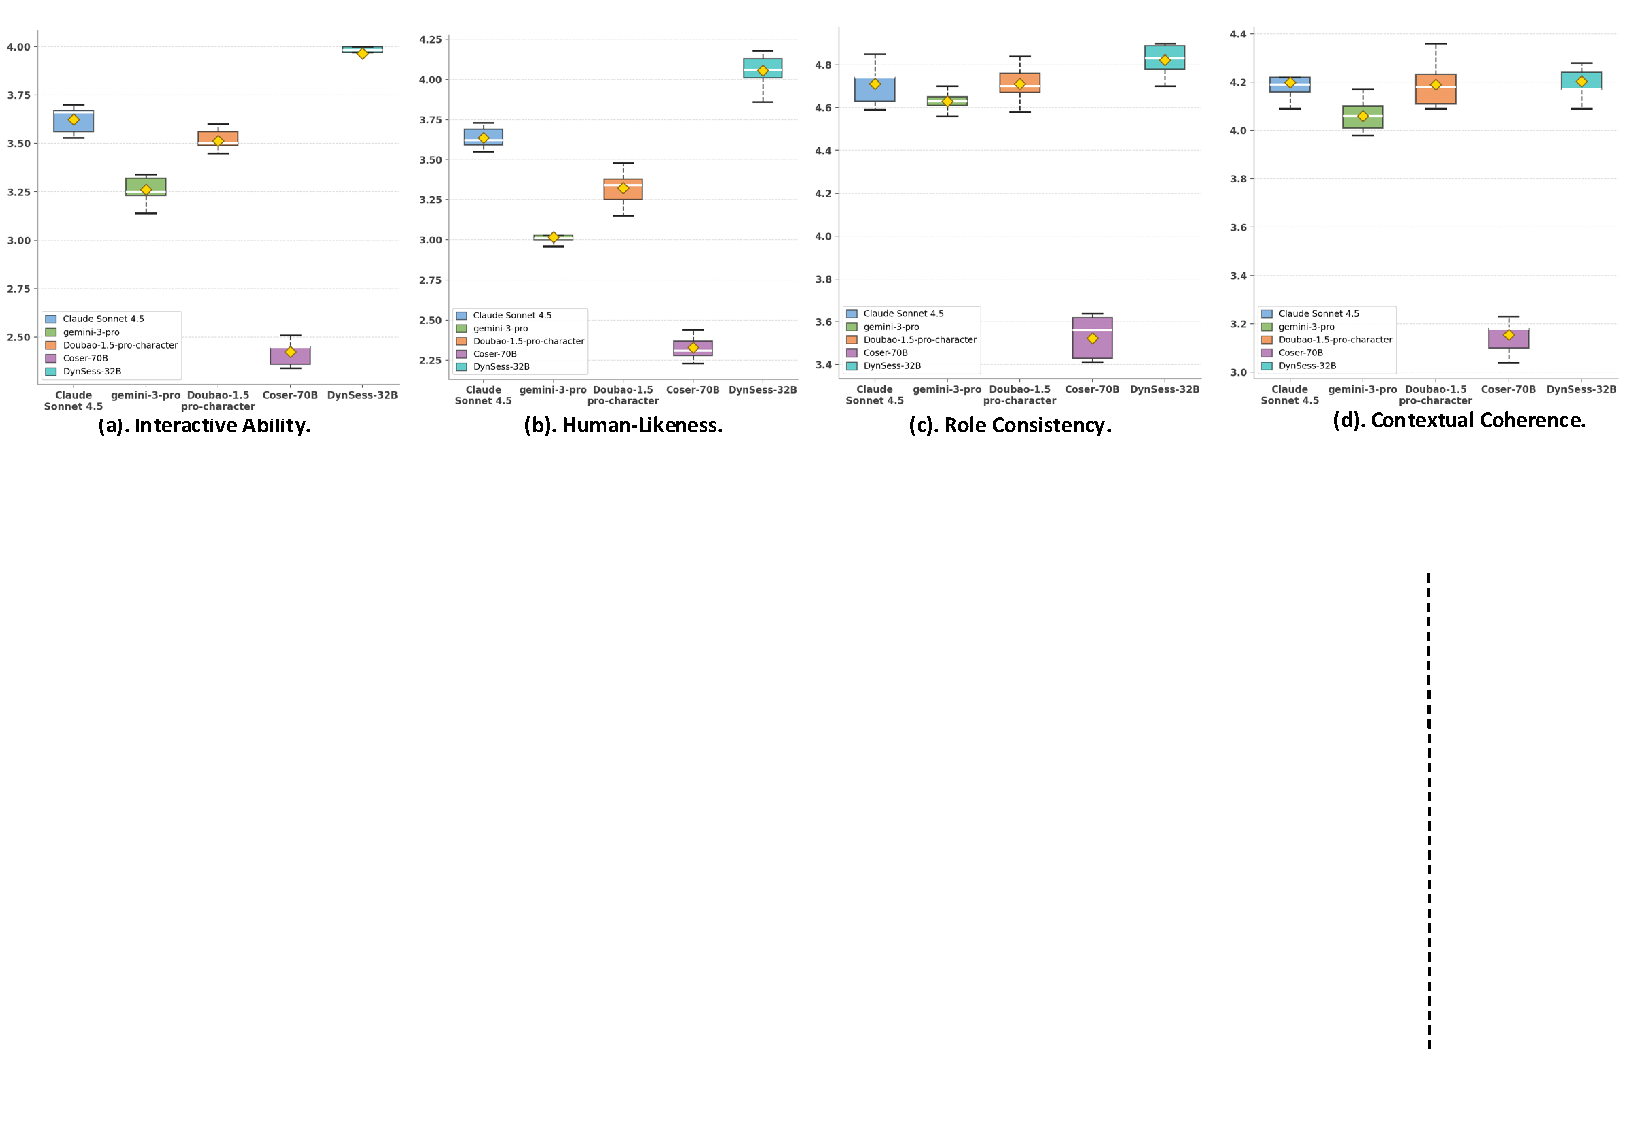
\includegraphics[width=\textwidth, trim = 0 11.5cm 0 0, clip]{latex/Image/appendix-experiment-analysis-bias-v1.pdf}

%   \caption{A figure with a caption that runs for more than one line.
%     Example image is usually available through the \texttt{mwe} package
%     without even mentioning it in the preamble.}
%   \label{fig:experiments}
% \end{figure*}


% --更多case study，eval prompt，user prompt生成的prompt，用户模拟器prompt， 
% \subsection{Others}

